\chapter{test setting}
In this study the peripheral circulation is observed to investigate if there are changes in microcirculation during partial occlusion of blood supply. Infrared imaging is used to measure the temperature changes in the skin of the hand, which is used as an indicator for peripheral circulation. 
To see if there are changes in the microcirculatory system depending on flow levels in the macrocirculatory system, the test is set in two conditions. The first measurement of the hand, which is done under normal conditions, is used as a control measurement. The second measurement of the hand is done during a partial occlusion of the blood supply. The partial occlusion of the arm leads to an ischemia, which leads to a lower oxygen supply and is used as a way to mimic sepsis, which also leads to lower oxygen supply. \fxnote{introduce why 50\% of blood flow}

<<<<<<< HEAD
By first taking the control measurement under normal conditions, the carry-over effect of the occlusion is avoided. It also enables to take both measurements of each subject straight successively, what reduces inaccuracies within the setup of both experiments for each subject. Therefore a special setting, which is shown in \cref{fig:setting} is assembled in the Regionshospital Nordjylland in Hj\o{}rring.
=======
By fist taking the control measurement under normal conditions, the carry-over effect of the occlusion is avoided. It also enables to take both measurements of each subject straight successively, what reduces inaccuracies within the setup of both experiments for each subject. Therefore a special setting is assembled in the Regionshospital Nordjylland in Hj\o{}rring.

The subject will be placed in a upholstered chair with adjustable backrest, footrest and also armrests, which allows a good positioning of the measured hand. The measured hand is the dominant hand and must be fixed during the whole test to minimize movement bias. Hence the hand is stabled with a vacuum pillow which is covered by a micro fiber tissue to get a better background for the images. To provide a more comfortable position of the arm during the experiment the armrest of the adjustable chair is padded with some sheets under the vacuum pillow. A comfortable position in the chair is important, because the subject has to sit still and is not allowed to move during the test for at least 45 min, because the test setting just prevents very small unintentional movements.
$37,5\pm 1,0 cm$ over the hand the Xenics Gobi $640 17\mu$ m GigE infrared camera is positioned with a tripod. The focus is adjusted on the hand until the wrist.
The camera is via a Ethernet cable connected with a laptop, which is used to record the measurements with Xenics software with a frame rate of $ \frac{50}{8} \frac{1}{s} $ and to save the files. It should be respected, that the file has to be named or rather renamed before each recording, otherwise the software will overwrite the previous file.
>>>>>>> ee04b1bfa8286fb6bd3406c7bdf62c75486e3ec1

\begin{figure}[H]
	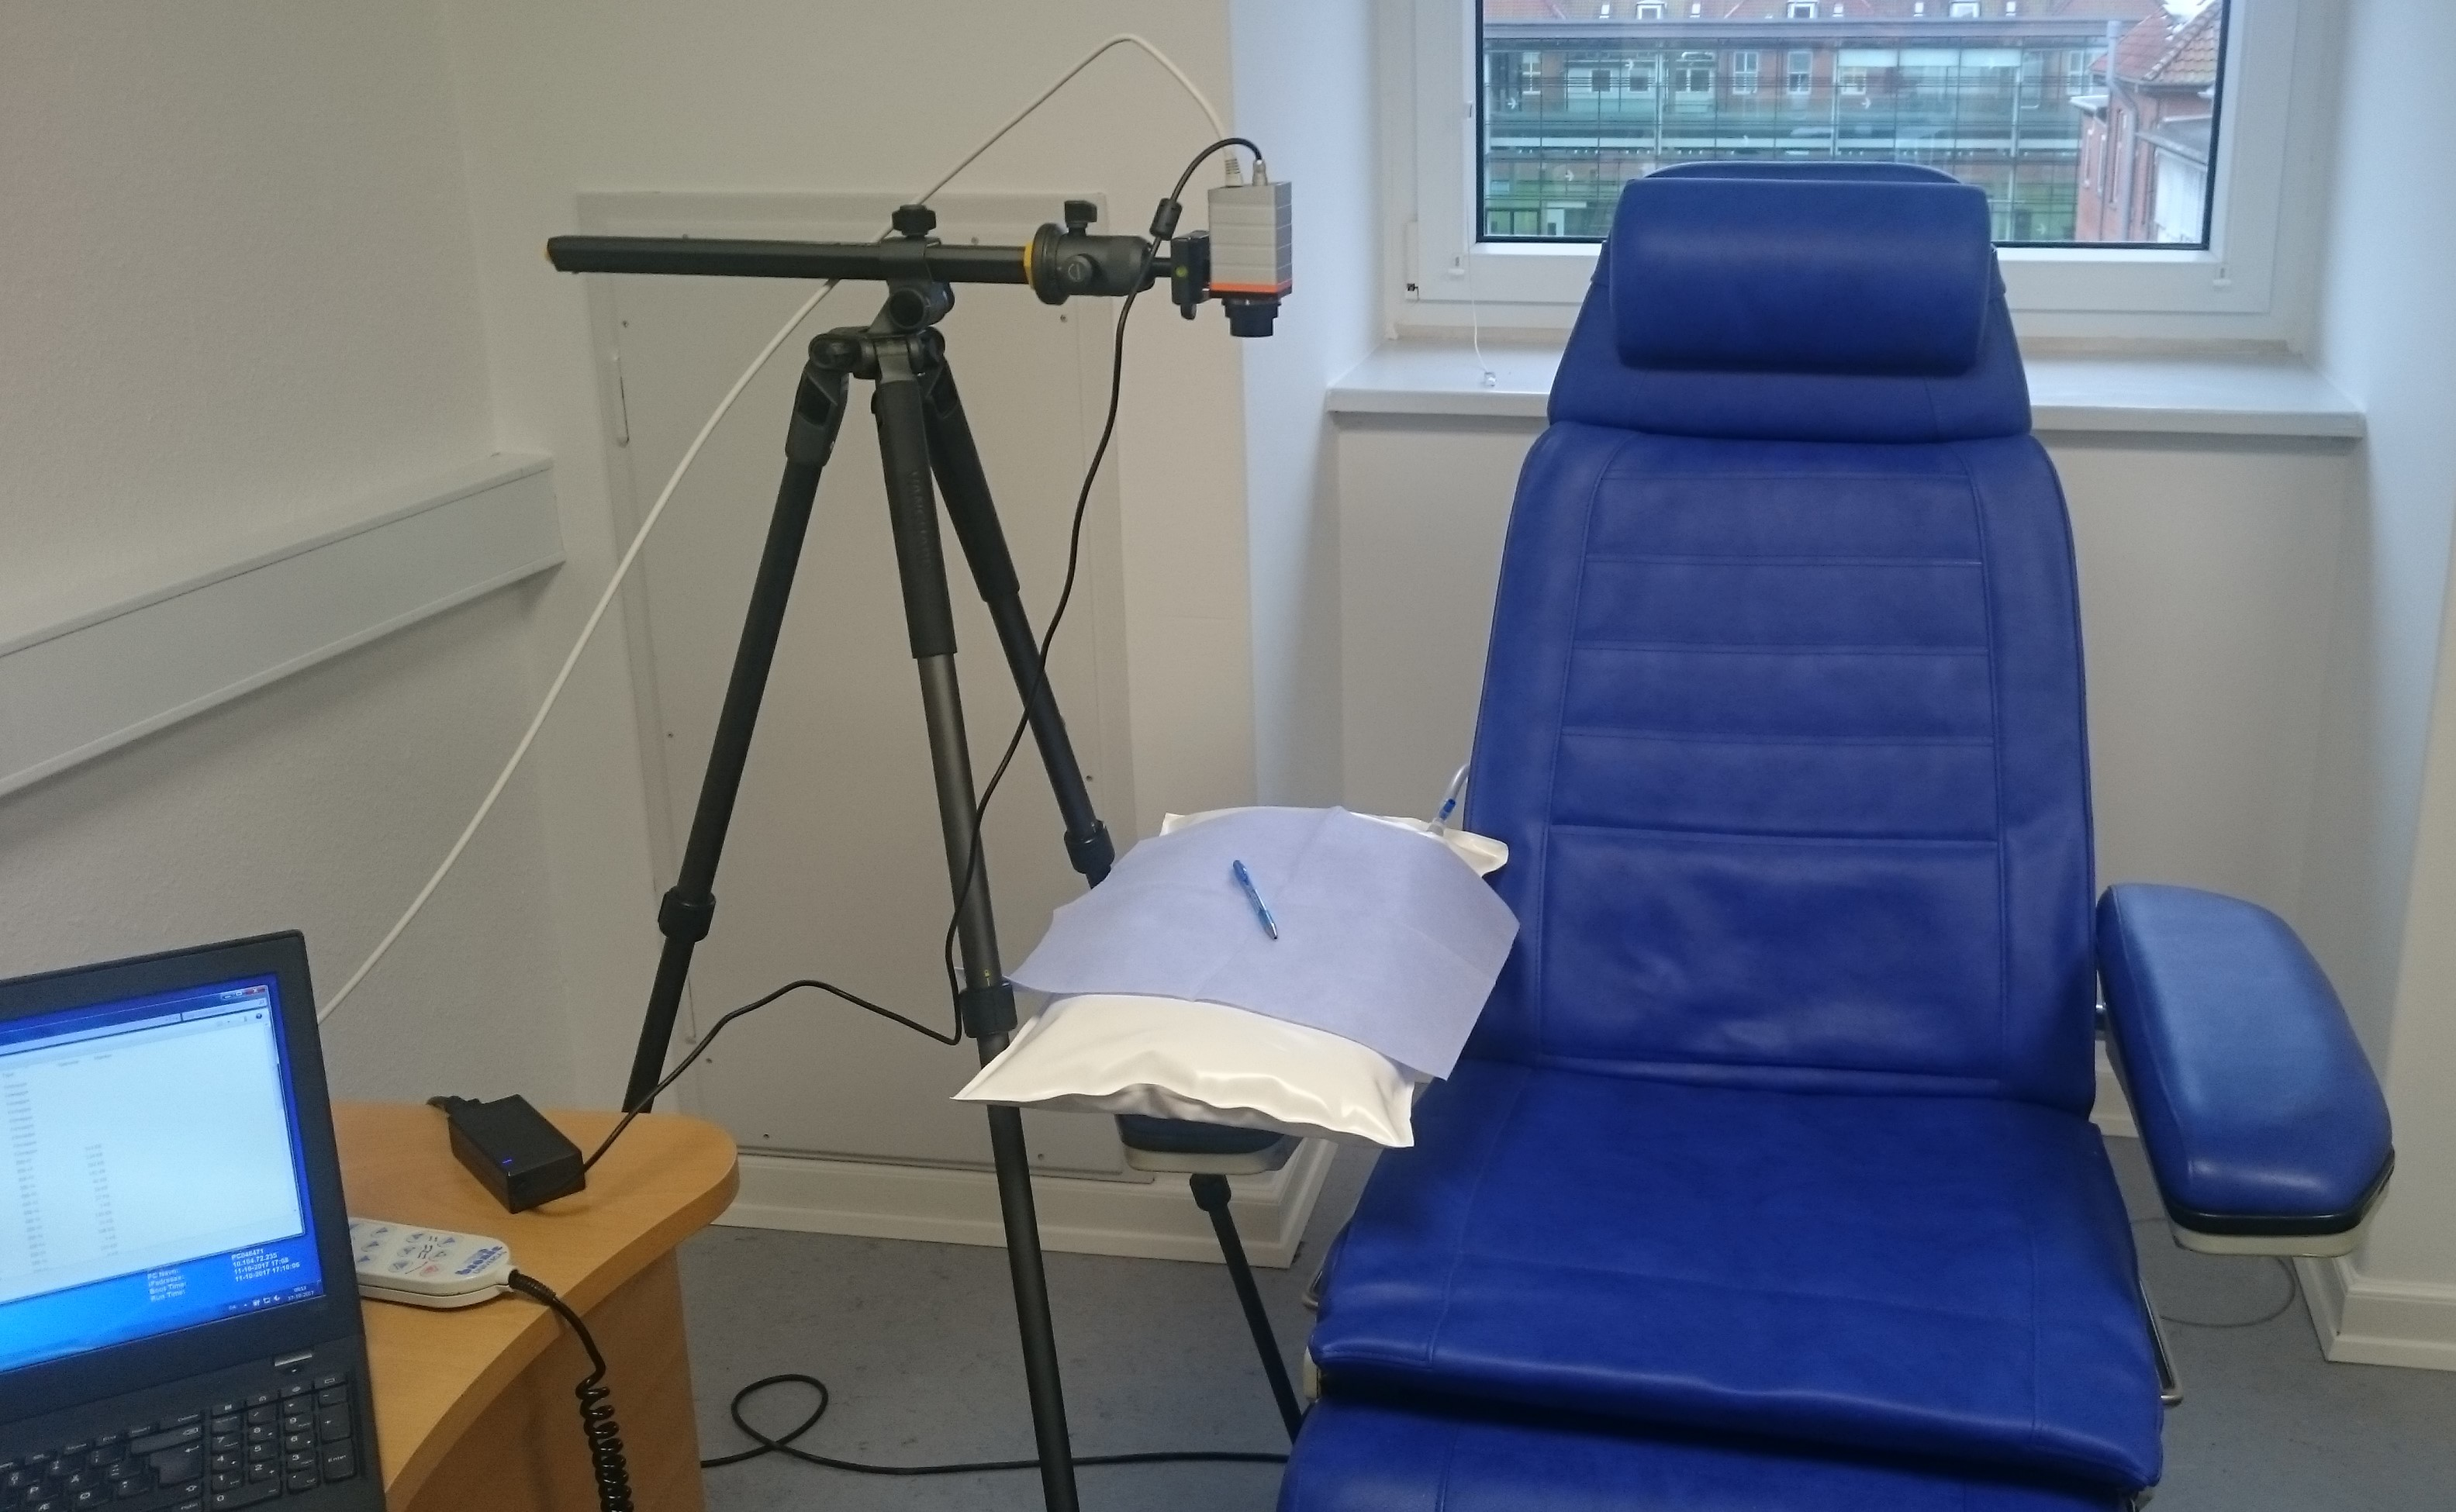
\includegraphics[width=0.7\textwidth]{figures/setting}
	\caption{The test setting in the Regionshospital Nordjylland.}
	\label{fig:setting}
\end{figure}
\fxnote{explanations of pic}

The subject will be placed in a upholstered chair with adjustable backrest, footrest and also armrests, which allows a comfortable positioning of the subject during the experiment. Measurements will be done on the dominant hand, which must be stabilized during the whole test to minimize movement bias. Hence the hand is stabled with a vacuum pillow which is covered by a micro fiber tissue to get a better background for the images, because microfiber \fxnote{look it up}. To provide a more comfortable position of the arm during the experiment the armrest of the adjustable chair is padded with some sheets under the vacuum pillow. A comfortable position in the chair is important, because the subject has to sit still and is not allowed to move during the experiment for at least 45 min, because the test setting just prevents very small unintentional movements.
The Xenics Gobi 640 17\mu m GigE infrared camera is positioned with a tripod over the hand. Focus is adjusted on the hand until the wrist \fxnote{rewrite this sentence!}.
The camera is via a Ethernet cable connected with a laptop, which is used to record the measurements with Xeneth software with a frame rate of $ \frac{50}{8} \frac{1}{s} $ and to save the XVI-files. Before each measurement is started, a unique file name has to be chosen and typed in, otherwise the software will overwrite the previous file.

First the cable connections between the camera, the laptop and the power supply have to be set. Afterwards the camera is turned on and has to warm up for about 15 min. During this the laptop should be started and the software for taking the measurements is set in operational readiness. \fxnote{describe setting of camera (ambient temperature, emissivity,..)}

When the preparation of the test setting is done, the preparation for the subject can begin. At first the blood pressure of the subject is measured on the dominant arm. The blood pressure is measured three times while the subject is sitting relaxed on a chair. Out of the three measured systolic blood pressures the mean is calculated. To get the total occlusion pressure $(TOP)$ the mean has to be multiplied by 1,3. To reduce the blood flow in the arm to 50\% during the measurement within the second condition, the arm is cuffed with 30\% of the $TOP$ \cite{mouser2017}. The occlusion pressure that is applied in the cuff has also to be calculated before the experiment can start.
Then the cuff is affixed at the subjects dominant arm without tighten it. After that the subject can take place in the chair and the hand can be stabled with the vacuum pillow. The vacuum generator is attached to the pillow for giving the hand more stability. Next the camera needs to be positioned $37,5\pm 1,0 cm$ over the hand. The focus has to be adjusted. \fxnote{focus of lens, why?}

If the camera is stable and the filename is modified according to the subject, the first measurement can be started for 20 min. The time needs to be measured by a stopwatch. During the whole experiment the subject is not allowed to move or speak to minimize movement bias.
Directly after the first measurement the cuff on the arm of the subject is tightened with the calculated value $P_{cuff}=0,3\times TOP$ and the second measurement can be started for 20 min.The pressure of the cuff should be observed during the whole measurement and if necessary adjusted.

After the measurement of a subject, the next subject can be measured without preparing the test setting. It can be started with the preparation for the subject. It will take approximately one hour for each subject. For a guide during the experiment is an experimental protocol used.

XXX maybe an other picture
